% !Mode:: "TeX:UTF-8:Main"
% arara: pdflatex
% arara: convert: {density: 160, otheroptions: -dispose previous -delay 10 -loop 1, format: gif}
% arara: showfile: {format: gif}
\documentclass{article}
\usepackage[utf8]{inputenc} %probably not needed ...
\usepackage[T1]{fontenc}
\usepackage{geometry}
\geometry{papersize={128mm,96mm},margin=0.5cm} %\textwidth=11.8, \textheight=8.6
\usepackage[svgnames,x11names]{xcolor}
\usepackage[osf]{AlegreyaSans}
\usepackage{eso-pic}
\usepackage{xfp}
\usepackage{tikz}
\usetikzlibrary{shapes.geometric}
\usetikzlibrary{%
  shapes,
  decorations.shapes,
  decorations.fractals,
  decorations.markings,
  shadows
}

\usepackage{tikzducks}


\begin{document}
\AddToShipoutPictureBG{%
 \AtPageLowerLeft{%
 \begin{tikzpicture}[overlay,remember picture]
 \fill[Seashell1] (0,0) rectangle (\paperwidth,\paperheight);

\fill[Firebrick3] (current page.north west) rectangle ([yshift=-0.5cm]current page.north east);

 \fill[Firebrick3,ultra thick,bend right,draw=Silver] ([yshift=2cm]current page.south west) to ([xshift=-2cm]current page.north) -- (current page.north west) -- cycle;

 \fill[Firebrick3,thick,bend left,draw=Silver] ([yshift=2cm]current page.south east) to ([xshift=2cm]current page.north)--
 (current page.north east) --cycle;

\fill[Firebrick3] (current page.north west) rectangle ([yshift=-0.5cm]current page.north east);



 \foreach \i in {1,2,...,25}
     \fill [white!80!blue,decoration=Koch snowflake,opacity=.9]
           [shift={(rnd*5-1,rnd*6+3.6)},scale=0.2]
           [%double copy shadow={opacity=0.2,shadow xshift=0pt,
           %shadow yshift=3*\i pt,
           %fill=white,draw=none}
           ]
        decorate {
          decorate {
            decorate {
              (0,0) -- ++(60:1) -- ++(-60:1) -- cycle
            }
          }
        };

\foreach \i in {1,2,...,25}
     \fill [white!80!blue,decoration=Koch snowflake,opacity=.9]
           [shift={(rnd*5+8.8,rnd*6+3.6)},scale=0.2]
           [%double copy shadow={opacity=0.2,shadow xshift=0pt,
           %shadow yshift=3*\i pt,
           %fill=white,draw=none}
           ]
        decorate {
          decorate {
            decorate {
              (0,0) -- ++(60:1) -- ++(-60:1) -- cycle
            }
          }
        };

 \foreach \i in {1,2,...,10}
     \fill [white!80!blue,decoration=Koch snowflake,opacity=.9]
           [shift={(rnd*4+3.4,rnd+8.6)},scale=0.2]
           [%double copy shadow={opacity=0.2,shadow xshift=0pt,
           %shadow yshift=3*\i pt,
           %fill=white,draw=none}
           ]
        decorate {
          decorate {
            decorate {
              (0,0) -- ++(60:1) -- ++(-60:1) -- cycle
            }
          }
        };

 \end{tikzpicture}}}

\mbox{}

\medskip

{\centering\Huge\sffamily
\bfseries\scshape

Back\\ to \\ the \\ Regular \\ Programme
\par}

\vfill
\strut
\end{document}
